\documentclass[main_conf.tex]{subfiles}

\begin{document}

Inicialmente la caja eléctrica tiene 4 botones, un par de encendido y
apagado general y el otro otro par para el control de la máquina en
específico (Ver Fig. \ref{caja_electrica_tapa}).

\begin{figure}[!t]
  \centering
  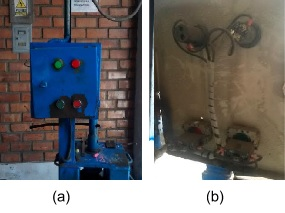
\includegraphics[width=3.0in]{../img/caja_electrica/tapa.jpg}
  \caption{Caja eléctrica (a) Vista exterior, (b) Vista interior}
  \label{caja_electrica_tapa}
\end{figure}

Estos botones se encuentran conectados a una llave termomagnética
y a arreglo de un contactor LC1D32 y un relé térmico de protección
LRD21.


\begin{figure}[t]
  \centering
  \begin{subfigure}[b]{0.5\textwidth}
    \centering
    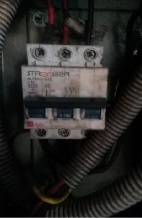
\includegraphics[width=1.5in]{../img/caja_electrica/llave_a.png}
    \label{caja_electrica_llave_a}
    \caption{Llave termomagnetica principal}
  \end{subfigure}
  
  \begin{subfigure}[b]{0.5\textwidth}
    \centering
    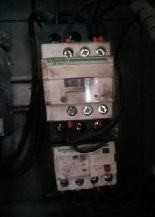
\includegraphics[width=1.5in]{../img/caja_electrica/llave_b.png}
    \label{caja_electrica_llave_b}
    \caption{Arreglo Contactor-Relé Térmico.}
  \end{subfigure}

  \caption{Llaves dentro de la caja eléctrica}
  \label{caja_electrica_llaves}
\end{figure}

La primera imagen muestra la llave termomagnética que se encarga del
control de energía a nivel general para todo el sistema, mientras que la
segunda nos enseña el arreglo que controla y protege al motor en caso de
una elevada corriente o temperatura.

El sistema de control de encendido de un motor monofásico utilizando
contactores es ampliamente conocido, como se muestra en la Fig.
\ref{diag_control_on_off_motor} por lo que parte de nuestro trabajo
consistirá en agregar un switch de apagado y encendido adicional que podrá
ser activado tanto de forma manual así como de forma automática y que en
la figura se encuentra sombreada como “Controla Distancia”.

\begin{figure}[t]
  \centering
  \begin{subfigure}[b]{0.5\textwidth}
    \centering
    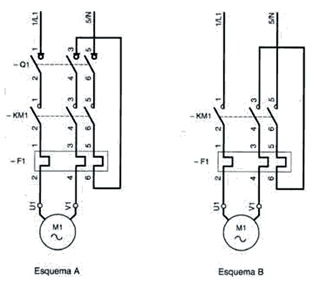
\includegraphics[width=2.0in]{../img/caja_electrica/Circuito_de_potencia.png}
    \label{Circuito_de_potencia}
    \caption{Circuito de Potencia}
  \end{subfigure}

  \begin{subfigure}[b]{0.5\textwidth}
    \centering
    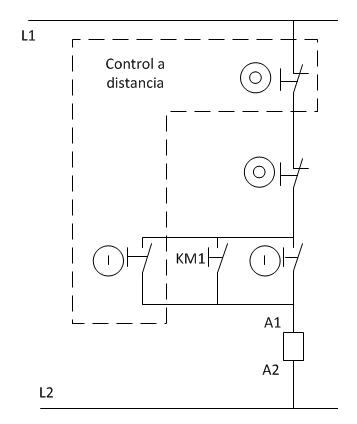
\includegraphics[width=2.0in]{../img/caja_electrica/Circuito_de_control.png}
    \label{Circuito_de_control}
    \caption{Circuito de control}
  \end{subfigure}

  \caption{Diagrama de circuital de encendido de un motor con contactor}
  \label{diag_control_on_off_motor}
\end{figure}

%
%\begin{figure}[!t]
%\centering
%\includegraphics[width=2.5in]{myfigure}
% where an .eps filename suffix will be assumed under latex,
% and a .pdf suffix will be assumed for pdflatex; or what has been declared
% via \DeclareGraphicsExtensions.
%\caption{Simulation Results}
%\label{fig_sim}
%\end{figure}

% Note that IEEE typically puts floats only at the top, even when this
% results in a large percentage of a column being occupied by floats.


% An example of a double column floating figure using two subfigures.
% (The subfig.sty package must be loaded for this to work.)
% The subfigure \label commands are set within each subfloat command, the
% \label for the overall figure must come after \caption.
% \hfil must be used as a separator to get equal spacing.
% The subfigure.sty package works much the same way, except \subfigure is
% used instead of \subfloat.


%\begin{figure*}[!t]
%\centerline{\subfloat[Case I]\includegraphics[width=2.5in]{subfigcase1}%
%\label{fig_first_case}}
%\hfil
%\subfloat[Case II]{\includegraphics[width=2.5in]{subfigcase2}%
%\label{fig_second_case}}}
%\caption{Simulation results}
%\label{fig_sim}
%\end{figure*}


% Note that often IEEE papers with subfigures do not employ subfigure
% captions (using the optional argument to \subfloat), but instead will
% reference/describe all of them (a), (b), etc., within the main caption.


% An example of a floating table. Note that, for IEEE style tables, the
% \caption command should come BEFORE the table. Table text will default to
% \footnotesize as IEEE normally uses this smaller font for tables.
% The \label must come after \caption as always.
%
%\begin{table}[!t]
%% increase table row spacing, adjust to taste
%\renewcommand{\arraystretch}{1.3}
% if using array.sty, it might be a good idea to tweak the value of
% \extrarowheight as needed to properly center the text within the cells
%\caption{An Example of a Table}
%\label{table_example}
%\centering
%% Some packages, such as MDW tools, offer better commands for making tables
%% than the plain LaTeX2e tabular which is used here.
%\begin{tabular}{|c||c|}
%\hline
%One & Two\\
%\hline
%Three & Four\\
%\hline
%\end{tabular}
%\end{table}
\end{document}
